
\section{Introduction}

\subsection{Problem Definition}

A \emph{content item} is some unit of information, such as a statement, graph,
table, example, and so forth.  An educationl television program, interactive
tutorial or university lecture (generally, these may all be called programs)
can be broken down into these units of information.  Call an item $\chi$; then
the $i^{th}$ item to be seen is $\chi_i$, and the time at which it is seen
$t_i$.  Then $(\chi_i, t_i)$ represents the $i^{th}$ item and its scheduled
time.  

For that matter, any program can be thought of as a sequence of these tuples,
thereby forming a schedule of items: 

\begin{equation}
\label{eq:schedule}
   X = \langle (\chi_1, t_1), (\chi_2, t_2), \ldots (\chi_n, t_n) \rangle.
\end{equation}
\vspace{2pt}

Furthermore $\chi$ could be a question, which could be thought of as an item
which accepts a response back that has a correct answer.  Items and questions
share many similar properties which help to distinguish them, such as the
ones in Fig~\ref{fig:properties}.

The main question this body of work seeks to answer is this: \emph{based on
input from the student on any subset of questions in an item schedule, how
should the remaining questions be scheduled}?

\subsection{Novel Contributions}

The answer to this question required a series of novel contributions to the
fields of intelligent tutoring systems (ITS) and computer-aided assessment
(CAT).  Specifically:

\begin{itemize}

 \item The creation of a data structure in the form of a graph, whose nodes
 contain information relevant to the assessment process, and whose edges
 capture dependency relationships among questions;

 \item A modification to an existing assessment theory known as Item Response
 Theory, which however providing a mature means of assessing student ability,
 benefited from an account of dependency relationships;
 
 \item A scheduler, or algorithm whose purpose was to determine what the
 questions should be given the item parameters and the students' response
 sets;

 \item An addendum to an existing theory of memory, forgetting, and practice,
 which could then be integrated into the scheduler to provide a fuller-featured
 system.

\end{itemize}

In addition to this, the body of work rests upon other incidental novel
contributions, such as the separation of Bloom level and difficulty
\cite{castleberry}.

\section{Bloom's Taxonomy}

Bloom's cognitive taxonomy organizes questions into levels depending on the
cognitive functions required of the answerer.  The levels are: knowledge,
comprehension, application, analysis, evaluation, and synthesis.  A brief
overview is given in Table~\ref{tab:bloom}, with definitions and examples of
questions covering the concept of for-loops:

\begin{table}
\label{tab:bloom}
\caption{The levels of Bloom's taxonomy defined}
\vspace{12pt}
\begin{tabularx}{\textwidth}{||l|X|X||}
\hline \hline
\rowcolor{Gray}
Level &  Explanation & Example Question \\\hline
Knowledge & Recalling factual information.   
& {What is a for-loop?}
\\ \hline
Comprehension & Assigning meaning to information.   
& {What does the example for-loop output? (Give example.)}
\\ \hline
Application & Applying a rule to a specific instance.   
& {How can the update statement of the loop be changed to print 
only even numbers?}
\\ \hline
Analysis 
& Breaking information into parts and exploring relationships.   
& {What would happen if the update statement decremented instead of incremented the counter?}
\\ \hline
Evaluation 
& Judging the use of knowledge or the validity of an
argument.   
& {Which is better for reading user input: a for-loop or a
while-loop? Why?} 
\\ \hline
Synthesis 
& Utilizing knowledge to create a new solution to
satisfy a goal.   
& {Write a for-loop to print only even numbers up to ten.}
\\ \hline \hline 
\end{tabularx}
\vspace{36pt}
\end{table}

Each category depends on the cognitive functions used in the previous category.
That is, comprehension requires knowledge, application requires comprehension,
and so forth.  Furthermore the mastery of one of the levels is with respect to
a given concept.  A student may be able to synthesize solutions to problems
dealing with expressions, but may not possess knowledge of equations, and thus
could not solve problems involving equations.

The utility of Bloom's taxonomy lies in its ability to pinpoint the underlying
cause of the student's problem-solving impasses \cite{shuhidan2011}.  Suppose a
test of mastery of loops is given with the comprehension question ``What does
such-and-such loop output?'' is given, and the student reaches an impasse.  If
the question ``What are the three expressions of the loop and what do they
do?'' is asked and the student does not know, the impasse can be attributed to
a lack of knowledge about loops.  If the student does know about the loop
expressions but still cannot answer, one might instead attribute it to a
comprehension difficulty \emph{as such}; which might be remedied by giving some
examples to build intuition, then continuing to test at the comprehension
level.

Educators may have an intuitive notion of how to do this, but Bloom's taxonomy
gives the ability to examine the impact of questions scientifically.  By
identifying the tested concept and the Bloom level of exercises, one can then
form hypotheses about student responses to questions.  

\subsection{The Interpretation in Computer Science}

Bloom's taxonomy has been proven to be useful at the undergraduate level, and
particularly in the field of software engineering \cite{britto2015,
mahmood2014}.  It has seen success in program comprehension
\cite{buckley2003}, where the asking of comprehension questions fosters code
reading \cite{losada2008}. In addition, it has been useful for pinpointing the
difficulties of novice programmers in a guided learning approach
\cite{shuhidan2011}.  It been used to identify a marked preference for
higher-level problems for those able to solve them \cite{bruyn2011}
\cite{goel2004}.  At least two experiments have shown the effect of item
ordering on performance \cite{newman1988effect,castleberry2016effect}, and the
taxonomy has even been applied to create ratings of courses based on the
average Bloom levels of tasks and questions in the course
\cite{oliver2004course}.

In spite of all this, there is an ongoing debate regarding the applicability of
Bloom's taxonomy to computer science \cite{johnson2006bloom,
fuller2007developing, thompson2008bloom}.  The crux of this debate centers
around the interpretation of Bloom levels: not only how questions map to Bloom
levels, but also regarding the progression of Bloom levels over the span of a
course or curriculum.  

A tacit assumption in much of the research is that Bloom levels equate to
difficulty levels.  While there is certainly a relationship between Bloom level
and difficulty in the ``ordinary course'' of devising problems, a distinction
can be made between the two.
% TODO: (SRB) cite the papers you cite in the difficulty paper regarding this assumption.

\subsection{Assumptions of this Work}

% TODO: (SRB) cite the prior research. I know it's not published yet.
Prior research by the author supports the view that Bloom level and difficulty
are separable parameters of a content item.  This work will proceed on the
assumption to that effect. 

In addition, some of the components of this body of work, particularly those
pertaining to memory and recall, are supported by many decades of empirical
research \cite{ebbinghaus}.  While the study of intelligent tutoring systems
has seen attempts to validate addendums to these theories which accommodate
re-activation of forgotten knowledge, none have undergone extensive empirical
testing as is typical for psychological models.  The components of this body of
work regarding re-activation introduce hypotheses.

% TODO: more on this

\section{Item Response Theory}

Here is introduced a mature assessment theory known as Item Response Theory, an
alternative to Classical Test Theory (CCT).  Whereas Classical Test Theory
assigns a student a grade based on the student's position in a distribution of
composite test scores, Item Response Theory accounts for item difficulty, item
discrimination, the probability of guessing the question correctly.

One of the main appeals of IRT is its incorporation of item difficulty.  As
will be shown later, this is pertinent to the interpretation of Bloom levels.  

According to Item Response Theory (IRT), the probability $p_i$ that a student
answers correctly the $i^{th}$ question on a test, is given by:

\begin{equation}
 \label{eq:irt}
  p_i(\theta_s) = \gamma_i + \frac{1-\gamma_i}{1+e^{\alpha_i(\theta-\beta_i)}}
\end{equation}

where:

\begin{itemize} 

 \item $\alpha$ is the item discrimination, or how well the item can
 distinguish students of varying trait ability;

 \item $\beta$ is the question difficulty, an initial estimate of which can be
 obtained from the proportion of students with average trait ability who pass
 the question;

 \item $\gamma$ is the probability of guessing the answer correctly,
 which for $n$-choice questions is $1/n$;

 \item and $\theta$ is the \emph{trait ability} of the student, or the
 student's particular ability to answer that question correctly.

\end{itemize} 

A graph of the IRT curve for the parameters $\alpha=1, \beta=0, \gamma=0$ is
shown \ref{fig:irt}.

\begin{figure}[p!]
 \label{fig:irt}
 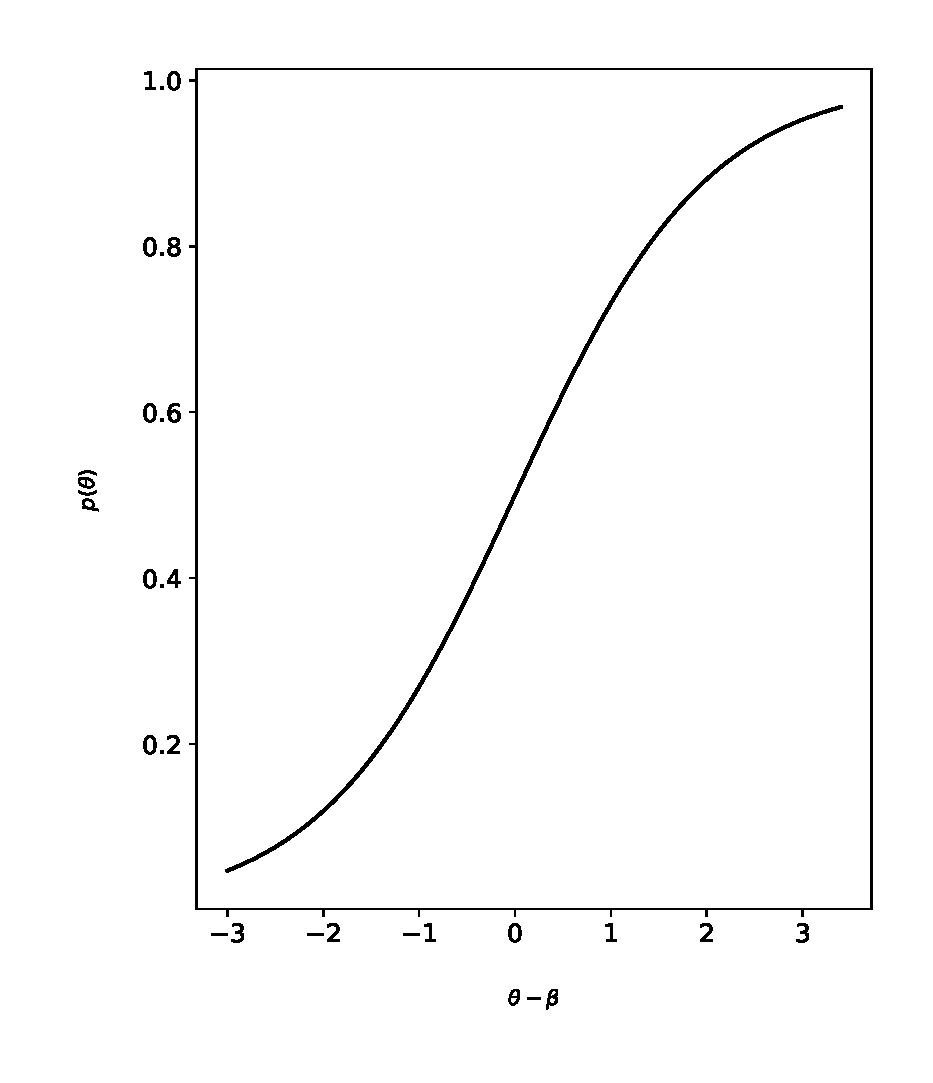
\includegraphics{fig/irt.eps} 
 \caption{A probability curve in Item Response Theory.}
\end{figure}

Note that $\alpha_i$, $\beta_i$, and $\gamma_i$ are parameters of the item $i$;
however $\theta_s$ is particular to the student $s$.  If the trait ability of
the student is known in addition to the item parameters, then the probability
of a correct response can be calculated.  However, it is more often than not
the case that the response set of the student is known, and trait ability is
unknown.  In such a case, a variety of techniques are deployable.

Trait ability in IRT can be obtained using a maximum likelihood estimation
(MLE) method, which finds a maximum-likelihood estimate of $\theta$ by testing
a range of $\theta$ values with the IRT formula \cite{baker2004}.  Later it
will be shown how $\theta$ can be estimated.  Another potential technique is
Newton-Raphson, which in most other applications would be the more efficient
and desirable method.  It will later be discussed why the MLE method is
preferred.

%The utility of IRT is that it requires fewer questions to gauge trait ability
%due to its account of other factors ($\alpha, \beta, \gamma$). It is thus
%reputed to be a more mature means of assessment than CTT.

Until now, the fusion of IRT and Bloom's taxonomy has only existed in the
literature as a possibility \cite{sitthisak}.  This work seeks to reconcile
the two by offering a compatible interpretation of Bloom's taxonomy.
%TODO: (SRB) I don't think this is true. See email I sent you on 1/24/2017.

\subsection{Evaluation of Trait Ability}

Consider a set of content items or questions for which the answer is either
incorrect or correct.  This is true in the case of multiple choice questions
(as well as true-false, which is a subset of multiple-choice questions).

Suppose the student has a response set for content items: 

\begin{equation}
  \label{eq:responses}
  X_s = x_{s1}, x_{s2}, \ldots, x_{si}, \ldots x_{sn}
\end{equation}

Here $X_s$ is the response vector of student $s$, and $x_{si}$ is the
correctness of the response to content item $i$ by student $s$; it is zero if
the response is incorrect, or 1 if it is correct.  

These questions may be of various and sundry discriminations, difficulties, and
probabilities of guessing.  The first question may have $\alpha_1=.5$,
$\beta_1=1$, and $\gamma_1=.25$; the second may only differ in its difficulty,
for example $\beta_2=-1$.  However, it shall be assumed that the set of
content items for which the student has provided responses are for the same
concept and the same Bloom taxonomic level.  The reason for this assumption
will become apparent later.

Recall that the probability $p_{si}$ of student $s$ answering the $i^{th}$
question correctly is:

\begin{equation}
  p_{si}(\theta_s) = \gamma + \frac{1-\gamma_i}{1+e^{\alpha_i(\theta-\beta_i)}}
  \tag{\ref{eq:irt}}
\end{equation}

Since $\theta_s$ is unknown but the response set is known, one method for
determining $\theta_s$ is by guessing all possible values.  First, one can
define a function $f_{si}$:

\begin{equation}
f_{si}(\theta_s) =\left\{
         \begin{array}{ll}
               p_i(\theta_s) & \mathrm{if}\  x_{si} = 1 \\
               q_i(\theta_s) & \mathrm{otherwise}
         \end{array}
       \right.
\end{equation}
% TODO: (SRB) Do you mean p_{si} above when you type p_i?

where 

\begin{equation}
   q_{si}(\theta_s)  = 1 - p_{si}(\theta_s).
\end{equation}

That is, $f_{si}$ assumes the probability $p_{si}$ if answered correctly and
$q_{si}$ if not answered correctly.  Proceeding on the assumption that each of
the observations (that is, responses in the response set) is independent, the
probablity of observing a total response set given a particular $\theta_s$
value is the product of the probabilities $f_{si}$ for all $i$, $1 \leq i \leq
n$, or

\begin{equation}
  \prod_{i=1}^n f_{si}(\theta_s).
\end{equation}

Supposing that there exists some $\theta_s$ which maximizes this product,
the most likely value for the student's true trait ability $\theta_s$ is
defined by:

\begin{equation}
  \theta_s = 
  \underset{\theta}{\textrm{argmax}}
  \Bigg[ 
  \prod_{i=1}^n f_{si}(\theta).
  \Bigg]
\end{equation}

that is, that value of $\theta_s$ which maximizes the product which gives the
probability of all the observations occuring together, given $\theta_s$.  To
obtain this, products for a range of possible $\theta$ values are calculated.

In the intelligent tutoring system which has been constructed, there are only
thirteen such values, drawing from the +/- system.  The mapping of grades to
trait ability levels is given in Table~\ref{tab:grades}.  This mapping could
also be applied to difficulty levels of questions.  A ``C question`` is one
which students of average trait ability (and perhaps just more than half the
class) may be expected to answer; an ``A+ question`` is a very difficult
question which students of only A+ ability at the time of asking may be
expected to answer; and an ``F question`` is one which may be used to determine
if a student's trait ability is minimally satisfactory.  This mapping lends to
a intuitive understanding of trait ability--as the familiar letter grade.  An
MLE may thereby effectively grade the student.
% TODO: (SRB) Is there some reason why you have ``C question`` instead of ``C question''?
% TODO: (SRB) Something should be said about the confidence in the trait ability assessment given above. In principle, a letter grade could be obtained from 2 questions.

\begin{table}[t]
\label{tab:grades}
\caption{Grades mapped to trait ability levels}
\vspace{12pt}
\begin{tabularx}{\textwidth}{||l|c|X||}
\hline\hline
\rowcolor{Gray}
Letter  & $\theta$  & Explanation \\\hline
F  & -3.0   & unsatisfactory \\\hline
D- & -2.5   &                \\
D  & -2.0   & minimal        \\
D+ & -1.5   &                \\\hline
C- & -1.0   &                \\
C  & -0.5   & acceptable     \\
C+ & 0.0    &                \\\hline
B- & 0.5    &                \\
B  & 1.0    & good           \\
B+ & 1.5    &                \\\hline
A- & 2.0    &                \\
A  & 2.5    & distinguished  \\
A+ & 3.0    &                \\\hline\hline
\end{tabularx}
\vspace{36pt}
\end{table}

To that end, rather than using a fine-grained MLE, it makes practical sense to
calculate products for these thirteen values of $\theta$, since higher
granularity than the +/- system is not useful for final grade assignment, nor
is necessarily more intuitive for the student or instructor.  Restricting the
products calculated to this set of values also makes sense from an efficiency
standpoint.  The total time complexity of the MLE is linear in the size of the
response set, regardless of the number of guesses in $\theta$; while not
asymptotically reduced from using a smaller step size, it is five times faster
than $10^{-1}$, and fifty times faster than $10^{-2}$.  A graph calculating
likelihoods for MLE is depicted in Figure~\ref{fig:mle}.

% Talk about gradient descent and Newton-Raphson

The total number of MLE estimations for trait ability throughout a course is
equal to the total number of responses for all questions throughout a course,
which can be quite large; it is proportional to the number of students times
the number of items. 

\begin{figure}[p!]
 \label{fig:mle}
 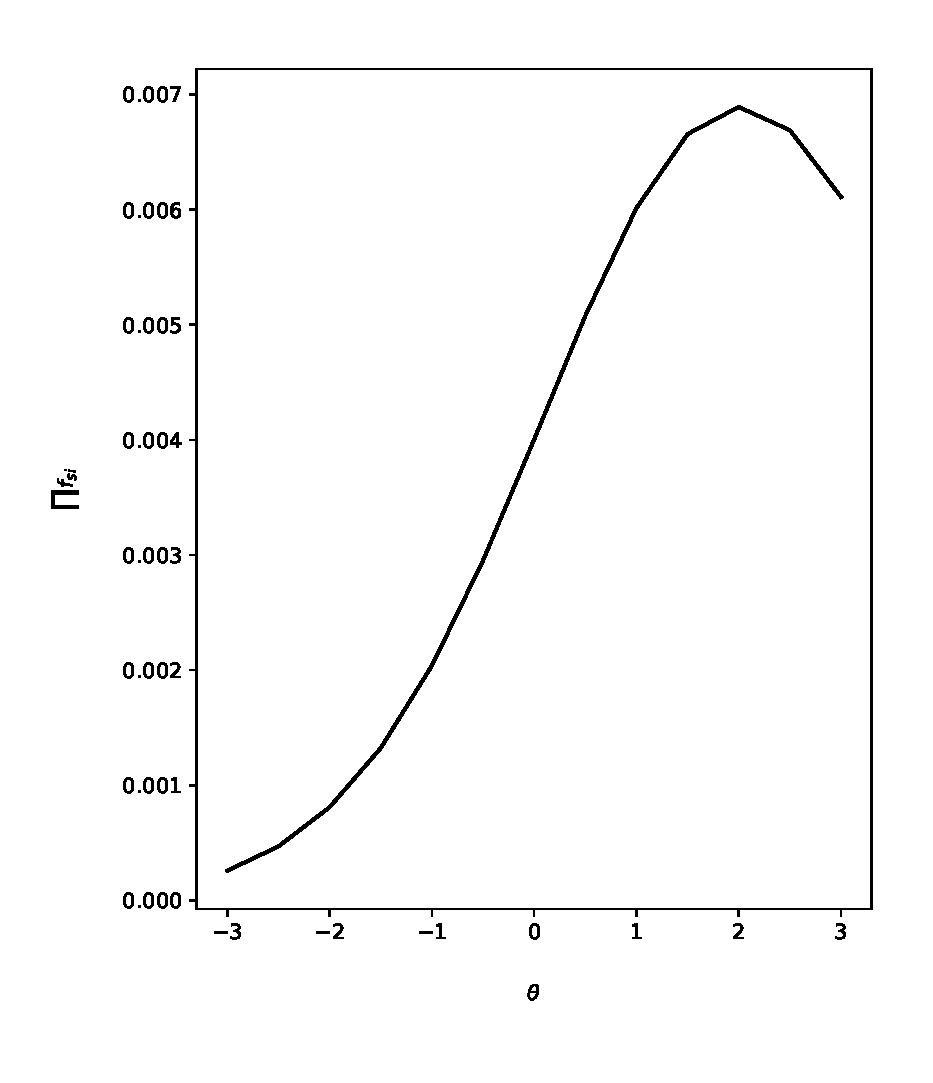
\includegraphics{fig/mle.eps} 
 \caption{A maximum-likelihood estimation for IRT}
\end{figure}

\section{Factor Analysis}

Suppose ${Y}$ is a vector of $m$ observed random variables.  It is
posited that there are $n : n \leq m$ latent, or hidden variables which explain
${Y}$, in addition to item-specific variables $\epsilon$.  ${Y}$
may be scores on test questions (what is directly measured); latent variables
may be degree of understanding, amount of time spent studying, alertness,
verbal intelligence, and so forth (what is indirectly measured).  An example
of a factor analysis diagram is given in Figure~\ref{fig:factors}.

This relationship may be expressed this using the following system of equations
\cite{mulaik2010}:

\begin{equation}
\begin{array}{ll}
\label{eq:factsystem}
  y_1  = & \lambda_{11} \zeta_{1}  +  \lambda_{12} \zeta_{2}  +  \ldots  \lambda_{1n} \zeta_{n}  +  \psi_1 \epsilon_1 \\
  y_2  = & \lambda_{21} \zeta_{1}  +  \lambda_{22} \zeta_{2}  +  \ldots  \lambda_{2n} \zeta_{n}  +  \psi_2 \epsilon_2 \\
  \vdots \\
  y_m  = & \lambda_{m1} \zeta_{1}  +  \lambda_{m2} \zeta_{2}  +  \ldots  \lambda_{mn} \zeta_{n}  +  \psi_m \epsilon_m \\
\end{array}
\end{equation}

Here, $\zeta$ represents a factor, or latent variable. The $\lambda$ weight
represents a factor loading, or extent to which the factor influences $y$;
$\epsilon$ is an item-specific random variable, and $\psi$ is its loading. This
above system may be expressed in matrix notation:

\begin{equation}
 \label{eq:factmatrix}
 {Y} = {\Lambda} {X} + {\Psi} {E}
\end{equation}

This is known as the fundamental equation of factor analysis. Here, ${\Lambda}$
is known as the loading matrix of the factors.  For normalized ${Y}$, it gives
the amount of variance accounted for by each factor in ${X}$.  

The means by which ${\Lambda}$ is obtained:

% TODO

It suffices to say that factor analysis involves the interpretation of
${\Lambda}$, and may be one of two types: confirmatory or exploratory.


\subsection{Confirmatory vs. Exploratory}

Confirmatory factor analysis (CFA) seeks to confirm that hypothesized factors
accounted for a certain threshold of variance. Exploratory factor analysis
(EFA) seeks to find factors which account for unexplained variance.

In this thesis, the use of CFA is to confirm that dependency relationships
among items exist.  It is also used to find the extent of variance accounted
for by those dependency relationships.

\section{Previous Research}

% TODO
